\documentclass[a4paper, 12pt]{article}

\usepackage{report}
\usepackage{tabularx}
\usepackage{algorithm}      % 也會帶入 float 套件，讓 [H] 可用
\usepackage{algpseudocode}
\usepackage{graphicx}
\usepackage{amsmath}
\usepackage{pdfpages}
\usepackage{caption}        % 提供 \captionof
\usepackage{amssymb}
\usepackage{listings}
\usepackage[most]{tcolorbox}
\usepackage[table]{xcolor}
\usepackage{multirow}
\usepackage{booktabs}

\renewcommand{\figurename}{Figure~}
\renewcommand{\tablename}{Table~}
\rfoot{Page \thepage\ of \pageref{LastPage}}

\title{\textbf{U2296 Digital System Laboratory}\\ \Large LAB-04: Introduction to Verilog}
\author{.}
\date{}

\begin{document}
\maketitle

% 用 \input 而非 \include：\include 會在每章前後強制換頁，報告會變成很多半空的頁面
\section*{1. Goal}
Learn the basics of the Verilog hardware description language and the ModelSim simulation flow: describe the logic gates AND, XOR and NOR with gate-level Verilog modules, verify them with a test bench, and compare the simulated waveforms with the truth tables.

\section*{2. Theory}

\subsection*{Hardware Description Language (HDL)}
A hardware description language is a computer-based language that describes the hardware of digital systems in textual form. It resembles an ordinary programming language such as C, but it is specifically oriented to describing hardware structures and the behavior of logic circuits. The two HDLs standardized by the IEEE are VHDL and Verilog; this lab uses Verilog.

\subsection*{Modeling Styles in Verilog}
\begin{itemize}[leftmargin=*]
    \item \textbf{Gate-level modeling} describes a circuit by specifying its gates and how they are connected to each other.
    \item \textbf{Dataflow modeling} describes the Boolean equations of combinational logic with continuous assignments using the keyword \texttt{assign} (e.g.\ \texttt{assign F = A \& B;}).
    \item \textbf{Behavioral modeling} uses procedural assignments with the keyword \texttt{always}, and is mostly used to describe sequential circuits.
\end{itemize}
The modules in this lab use gate-level modeling with the built-in primitive gates of Verilog (\texttt{and}, \texttt{nand}, \texttt{or}, \texttt{nor}, \texttt{not}, \texttt{buf}, \texttt{xor}, \texttt{xnor}).

\subsection*{Structure of a Module}
\begin{itemize}[leftmargin=*]
    \item \texttt{module} / \texttt{endmodule}: start and end of the module declaration. The name after \texttt{module} is an identifier, which must begin with a letter or an underscore.
    \item \texttt{input} / \texttt{output}: declare which ports are inputs and which are outputs.
    \item \texttt{wire}: an internal connection between gates or modules.
    \item Gate instance: \texttt{and g1(F, A, B);} --- the output is listed first, followed by the inputs; \texttt{g1} is an optional instance name.
\end{itemize}

\subsection*{Test Bench}
To simulate a circuit, inputs must be applied so that the simulator can generate an output response. An HDL description that provides this stimulus is called a \textit{test bench}. In its simplest form, it is a module containing a signal generator and an instantiation of the model to be verified. Useful syntax:
\begin{itemize}[leftmargin=*]
    \item \texttt{reg A = 1'b0;} --- a register holding a 1-bit binary value of 0.
    \item \texttt{\#250} --- wait 250 time units (ps in this simulation) before executing the next statement.
    \item \texttt{\#2000 \$stop;} --- stop the simulation after 2000 time units.
\end{itemize}

\subsection*{Truth Tables}
\begin{table}[H]
\centering
\small
\begin{tabular}{c c | c c c}
\toprule
\textbf{A} & \textbf{B} & \textbf{AND} ($A \cdot B$) & \textbf{XOR} ($A \oplus B$) & \textbf{NOR} ($\overline{A + B}$) \\
\midrule
0 & 0 & 0 & 0 & 1 \\
0 & 1 & 0 & 1 & 0 \\
1 & 0 & 0 & 1 & 0 \\
1 & 1 & 1 & 0 & 0 \\
\bottomrule
\end{tabular}
\captionof{table}{Truth tables of AND, XOR and NOR gates}
\end{table}

\section*{3. Instruments and Components}

\begin{table}[H]
\centering
\small
\begin{tabularx}{0.8\textwidth}{X r}
\toprule
\textbf{Instrument / Software} & \textbf{Quantity} \\
\midrule
Personal computer (lab PC) & 1 \\
Intel FPGA 17.0 (\texttt{C:/intelFPGA\_pro/17.0}) & 1 \\
ModelSim -- Intel FPGA Starter Edition 10.5c & 1 \\
Verilog source files: \texttt{and.v}, \texttt{xor.v}, \texttt{nor.v} & 3 \\
Test bench file: \texttt{test\_bench\_2var.v} & 1 \\
\bottomrule
\end{tabularx}
\end{table}

\section*{4. Procedure}
\begin{enumerate}[leftmargin=*]
    \item Open \textbf{ModelSim -- Intel FPGA Starter Edition} from the Start menu.
    \item Create the main logic Verilog scripts.
    \begin{itemize}
        \item \textit{File $\rightarrow$ New $\rightarrow$ Source $\rightarrow$ Verilog}, then type the module \texttt{func\_and} using the primitive gate \texttt{and}.
        \item Save it as \texttt{and.v} under the FPGA directory \texttt{C:/intelFPGA\_pro/17.0/data/}.
        \item Repeat for \texttt{func\_xor} (\texttt{xor.v}) and \texttt{func\_nor} (\texttt{nor.v}).
    \end{itemize}
    \item Compile each script (\textit{Compile $\rightarrow$ Compile\ldots}, library \texttt{work}) and check the Transcript window for errors.
    \item Create a test bench \texttt{test\_bench\_2var.v}.
    \begin{itemize}
        \item Include the three source files with \texttt{`include}.
        \item Define module \texttt{tb\_func} and instantiate \texttt{func\_and}, \texttt{func\_xor} and \texttt{func\_nor} as \texttt{M1}, \texttt{M2} and \texttt{M3}.
        \item Change the inputs every 250 ps through the combinations $AB = 00 \rightarrow 01 \rightarrow 10 \rightarrow 11$, and stop the simulation at 2000 ps.
    \end{itemize}
    \item Compile the test bench. In the Library window, expand \texttt{work}, right-click \texttt{tb\_func} and select \textit{Simulate}.
    \item In the \texttt{sim} window, right-click \texttt{tb\_func} and select \textit{Add Wave}.
    \item Click \textit{Simulate $\rightarrow$ Run $\rightarrow$ Run -All} to generate the timing waveforms.
    \item Click on the wave window to read the signal values at a given time, and compare the simulation results with the truth tables.
\end{enumerate}

\newpage

\section*{5. Results Summary}
All three modules and the test bench compiled without errors. The simulated outputs below are read from the waveform in Figure~\ref{fig:wave}; ``Expected'' is the truth table from Section 2.

% 截圖原檔是整個 ModelSim 視窗 (1920x1040)，用 trim/clip 只裁出程式碼區，不改動原圖
% trim = 左 下 右 上 (單位 bp，PNG 無 DPI 資訊時 1 px = 1 bp)

\subsection*{AND Gate}
\begin{figure}[H]
    \centering
    \begin{minipage}[t]{0.48\textwidth}
        \vspace{0pt}
        \centering
        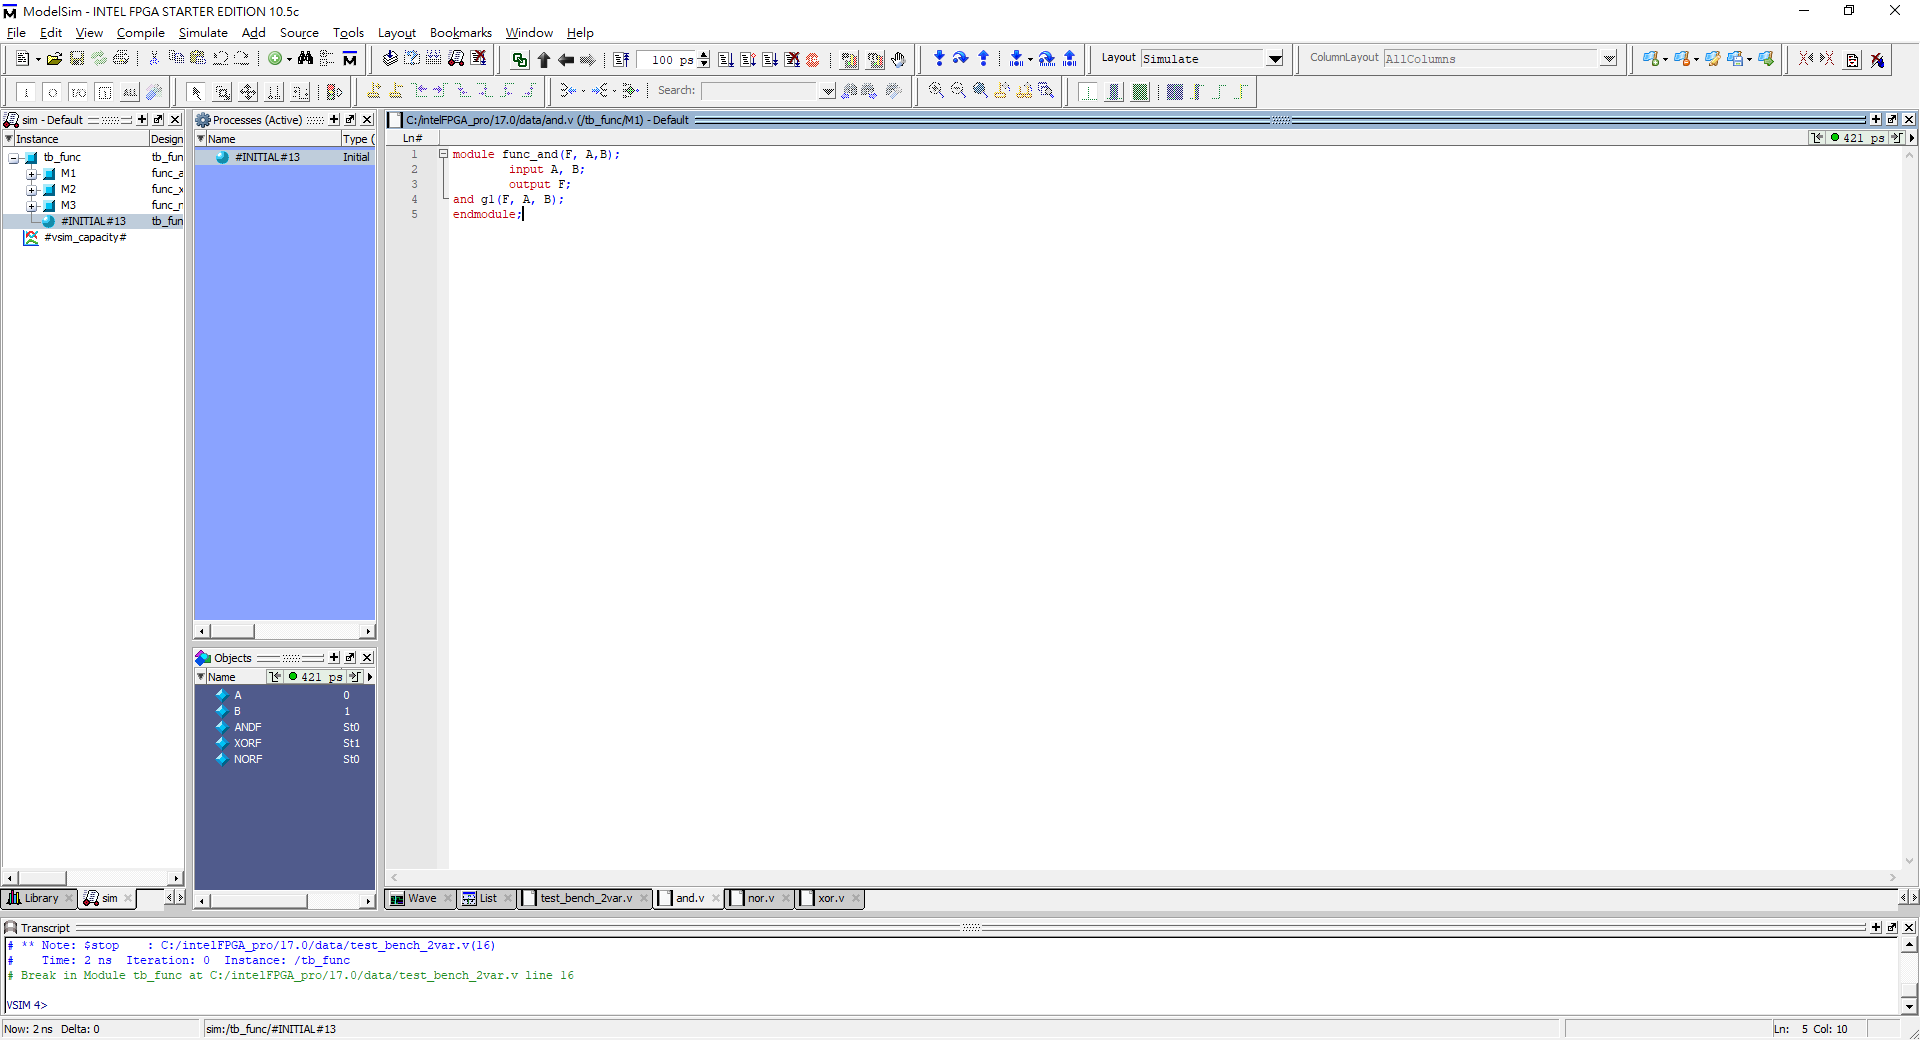
\includegraphics[width=\linewidth, trim=385 815 1160 112, clip]{pic/and.png}
        \captionof{figure}{\texttt{and.v} (module \texttt{func\_and})}
        \label{fig:and}
    \end{minipage}
    \hfill
    \begin{minipage}[t]{0.48\textwidth}
        \vspace{0pt}
        \centering
        \small
        \begin{tabularx}{\linewidth}{c c | >{\centering\arraybackslash}X | >{\centering\arraybackslash}X}
        \toprule
        \textbf{In A} & \textbf{In B} & \textbf{Expected} & \textbf{Simulated} \\
        \midrule
        0 & 0 & 0 & 0 \\
        0 & 1 & 0 & 0 \\
        1 & 0 & 0 & 0 \\
        1 & 1 & 1 & 1 \\
        \bottomrule
        \end{tabularx}
        \captionof{table}{AND gate truth table vs.\ simulation}
        \label{tab:and}
    \end{minipage}
\end{figure}

\subsection*{XOR Gate}
\begin{figure}[H]
    \centering
    \begin{minipage}[t]{0.48\textwidth}
        \vspace{0pt}
        \centering
        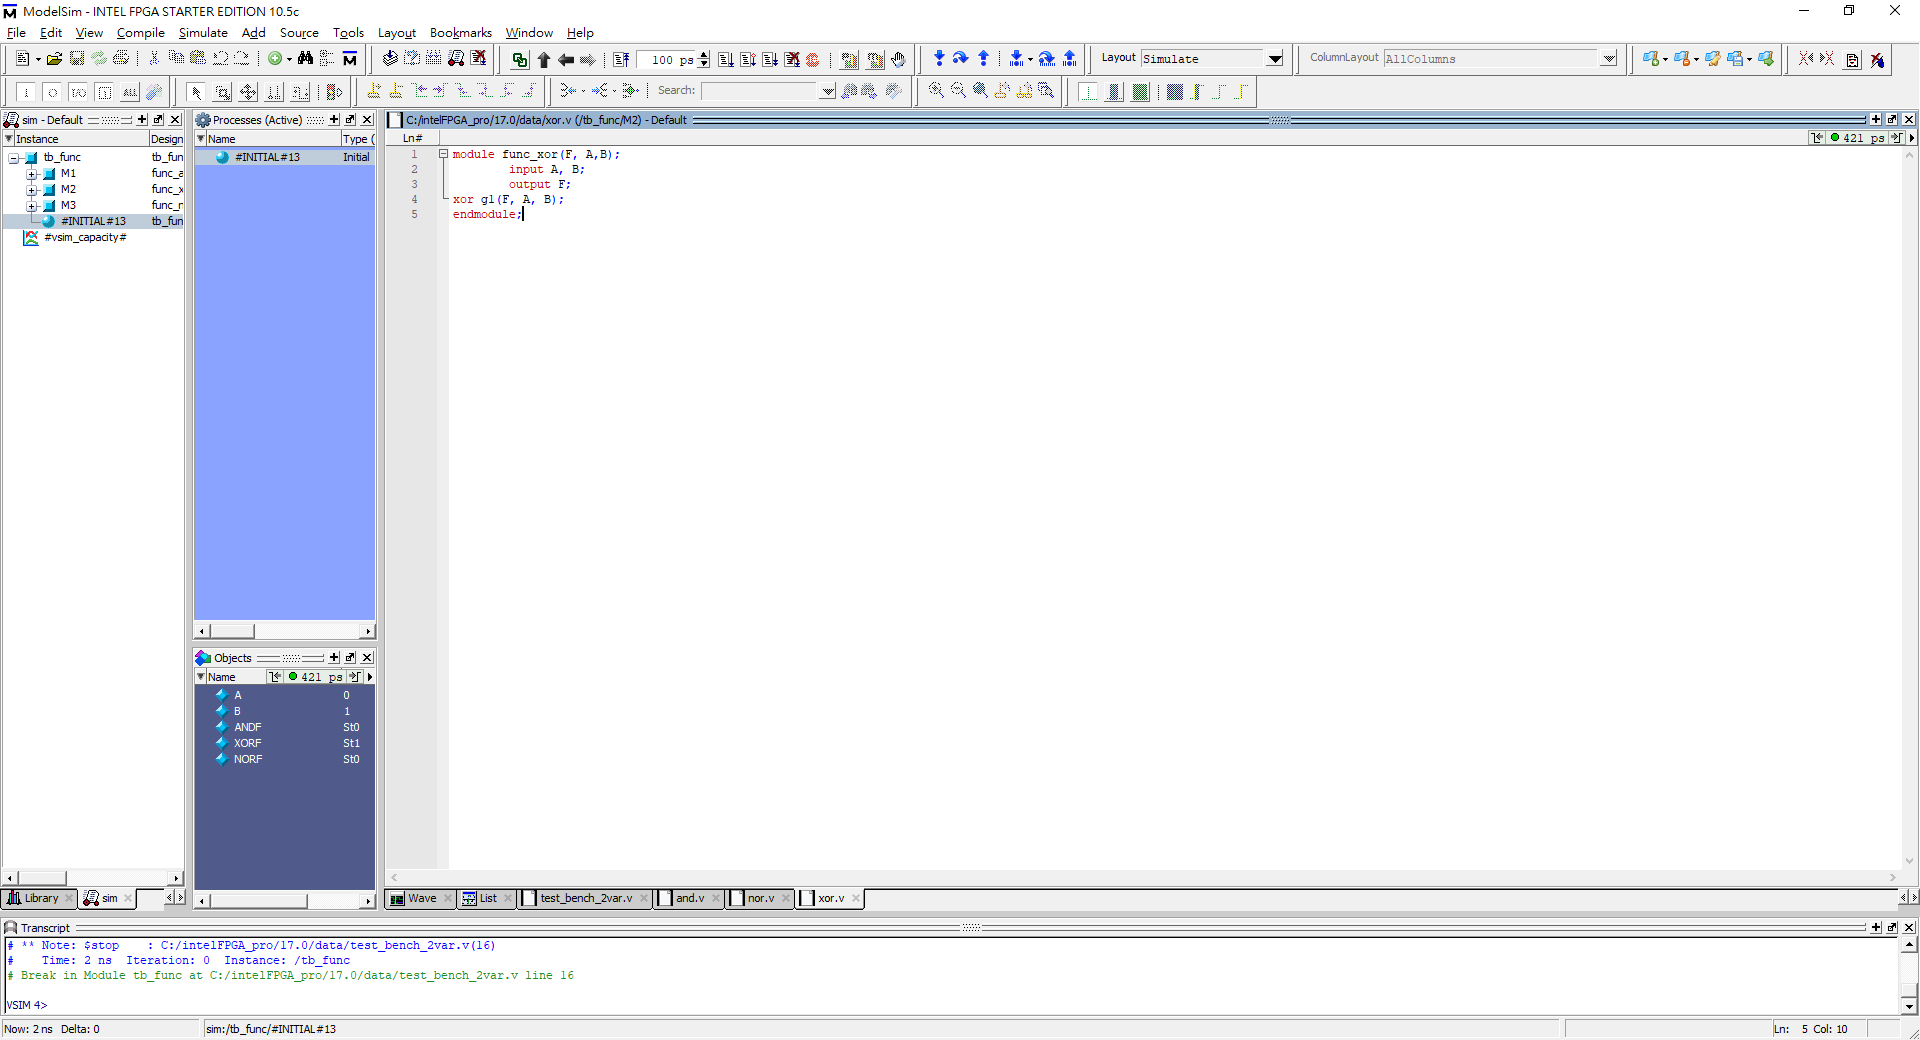
\includegraphics[width=\linewidth, trim=385 815 1160 112, clip]{pic/xor.png}
        \captionof{figure}{\texttt{xor.v} (module \texttt{func\_xor})}
        \label{fig:xor}
    \end{minipage}
    \hfill
    \begin{minipage}[t]{0.48\textwidth}
        \vspace{0pt}
        \centering
        \small
        \begin{tabularx}{\linewidth}{c c | >{\centering\arraybackslash}X | >{\centering\arraybackslash}X}
        \toprule
        \textbf{In A} & \textbf{In B} & \textbf{Expected} & \textbf{Simulated} \\
        \midrule
        0 & 0 & 0 & 0 \\
        0 & 1 & 1 & 1 \\
        1 & 0 & 1 & 1 \\
        1 & 1 & 0 & 0 \\
        \bottomrule
        \end{tabularx}
        \captionof{table}{XOR gate truth table vs.\ simulation}
        \label{tab:xor}
    \end{minipage}
\end{figure}

\subsection*{NOR Gate}
\begin{figure}[H]
    \centering
    \begin{minipage}[t]{0.48\textwidth}
        \vspace{0pt}
        \centering
        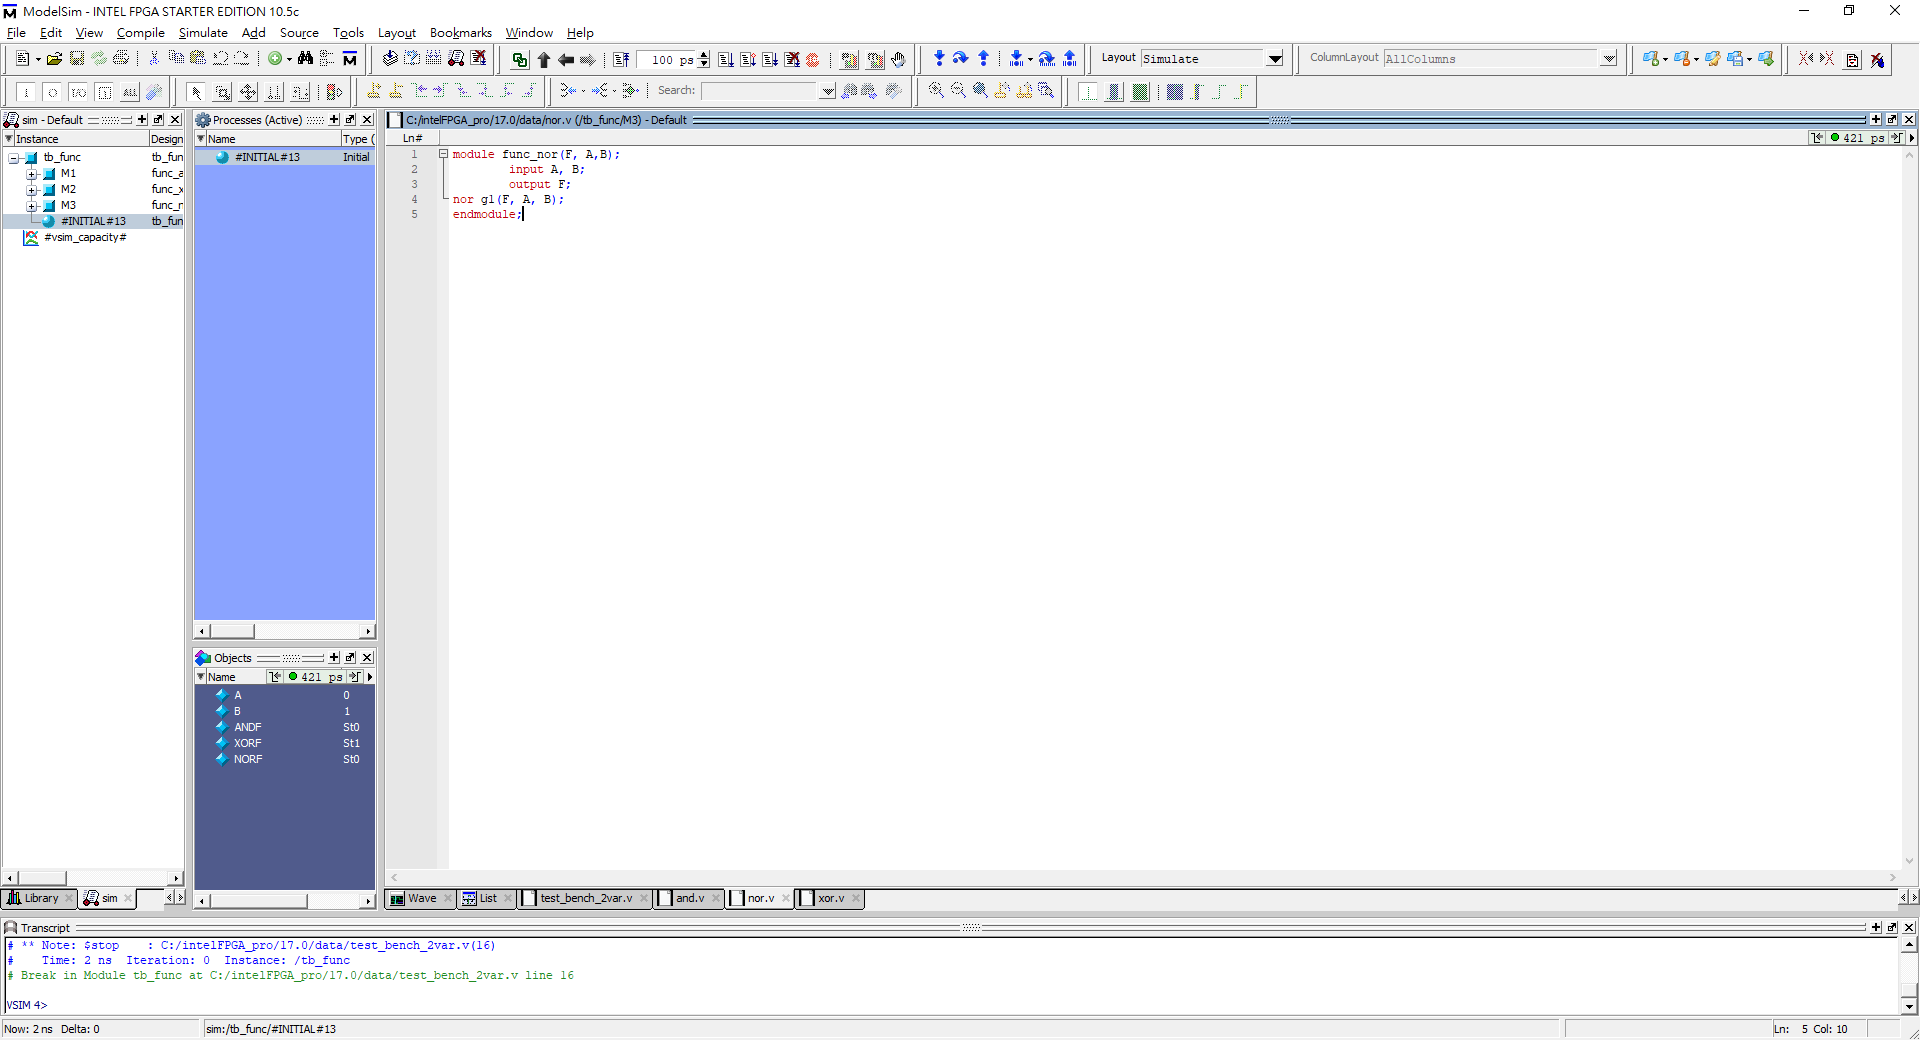
\includegraphics[width=\linewidth, trim=385 815 1160 112, clip]{pic/nor.png}
        \captionof{figure}{\texttt{nor.v} (module \texttt{func\_nor})}
        \label{fig:nor}
    \end{minipage}
    \hfill
    \begin{minipage}[t]{0.48\textwidth}
        \vspace{0pt}
        \centering
        \small
        \begin{tabularx}{\linewidth}{c c | >{\centering\arraybackslash}X | >{\centering\arraybackslash}X}
        \toprule
        \textbf{In A} & \textbf{In B} & \textbf{Expected} & \textbf{Simulated} \\
        \midrule
        0 & 0 & 1 & 1 \\
        0 & 1 & 0 & 0 \\
        1 & 0 & 0 & 0 \\
        1 & 1 & 0 & 0 \\
        \bottomrule
        \end{tabularx}
        \captionof{table}{NOR gate truth table vs.\ simulation}
        \label{tab:nor}
    \end{minipage}
\end{figure}

\subsection*{Test Bench}
The three modules are tested together in one test bench \texttt{tb\_func}: they share the inputs \texttt{A} and \texttt{B}, and drive the outputs \texttt{ANDF}, \texttt{XORF} and \texttt{NORF}.

\begin{figure}[H]
    \centering
    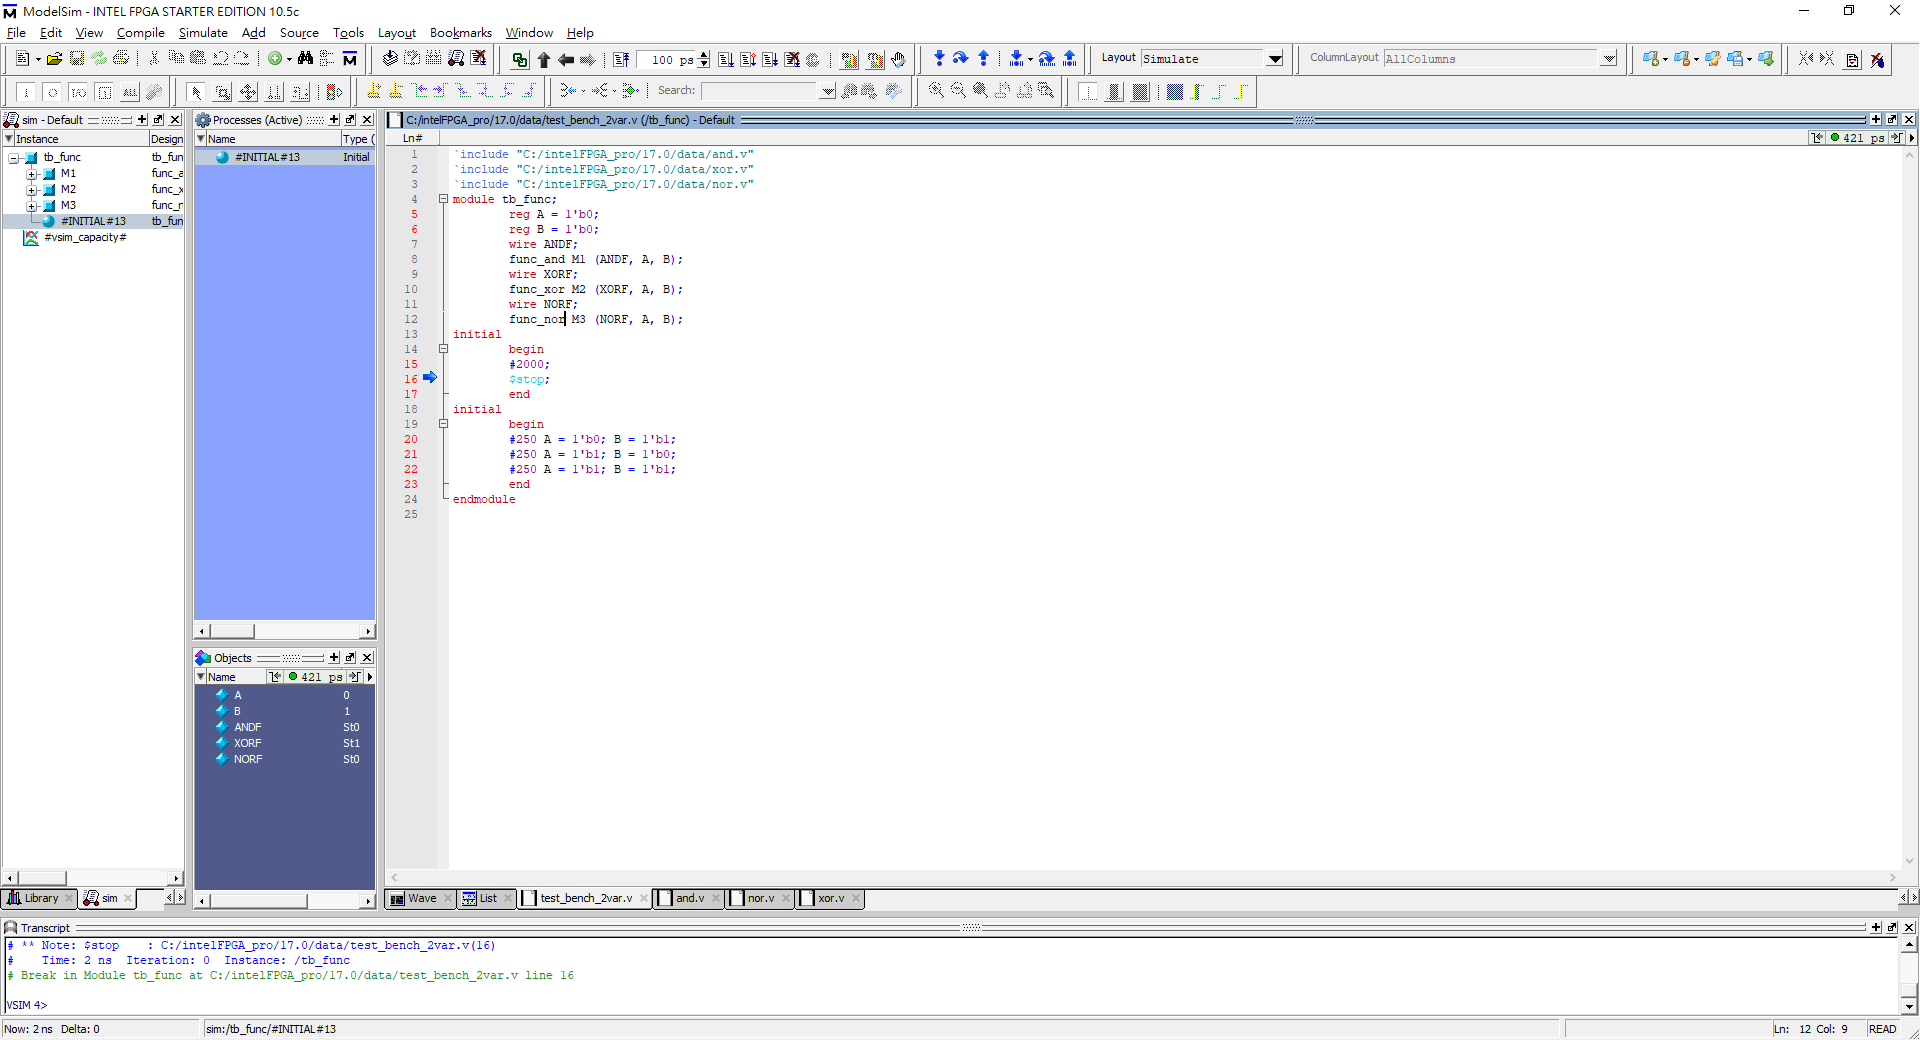
\includegraphics[width=0.6\textwidth, trim=385 532 1120 112, clip]{pic/test.png}
    \captionof{figure}{\texttt{test\_bench\_2var.v} (module \texttt{tb\_func})}
    \label{fig:tb}
\end{figure}

\subsection*{Simulation Waveform}
\begin{table}[H]
\centering
\small
\begin{tabular}{c c c | c c c}
\toprule
\textbf{Time (ps)} & \textbf{A} & \textbf{B} & \textbf{ANDF} & \textbf{XORF} & \textbf{NORF} \\
\midrule
0 -- 250    & 0 & 0 & 0 & 0 & 1 \\
250 -- 500  & 0 & 1 & 0 & 1 & 0 \\
500 -- 750  & 1 & 0 & 0 & 1 & 0 \\
750 -- 2000 & 1 & 1 & 1 & 0 & 0 \\
\bottomrule
\end{tabular}
\captionof{table}{Signal values read from the waveform}
\label{tab:wave}
\end{table}

\begin{figure}[H]
    \centering
    % 上段：訊號名稱與波形；下段：時間軸（中間全黑的空白區裁掉）
    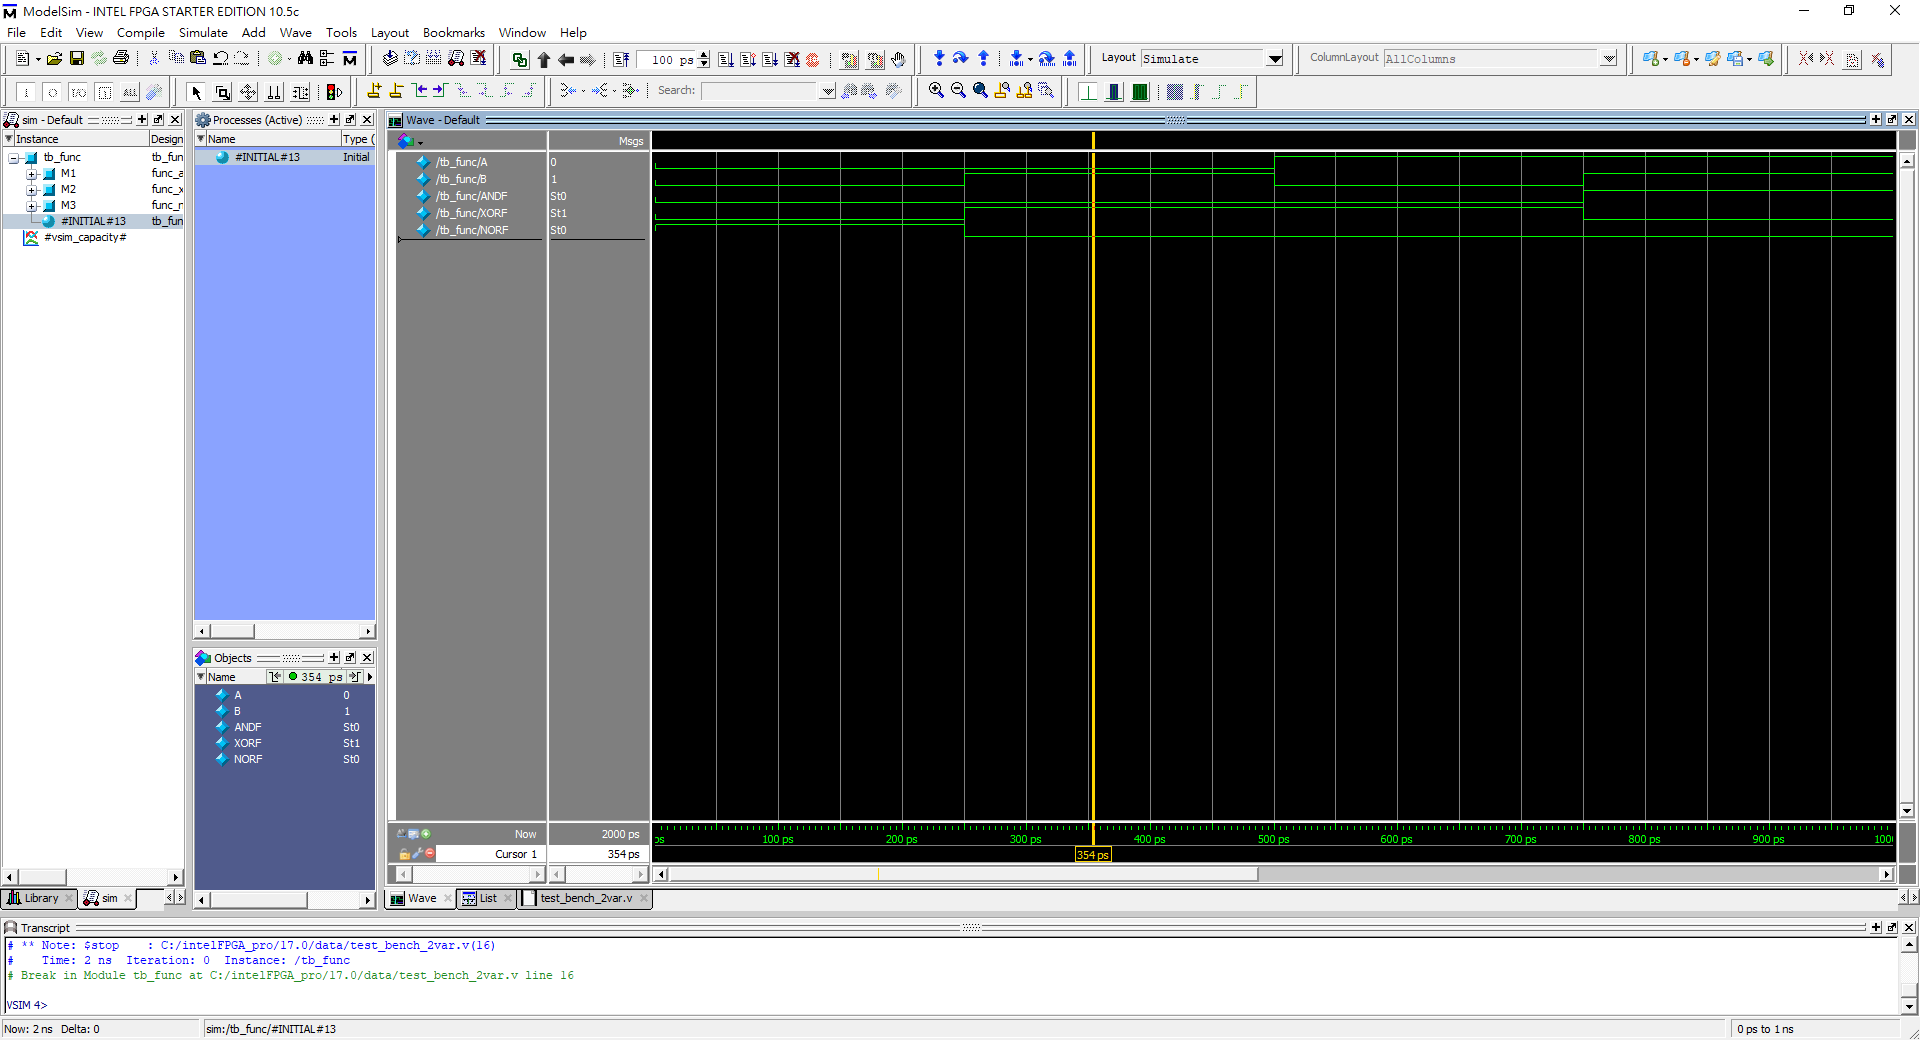
\includegraphics[width=\textwidth, trim=385 790 20 112, clip]{pic/result.png}\\[-1pt]
    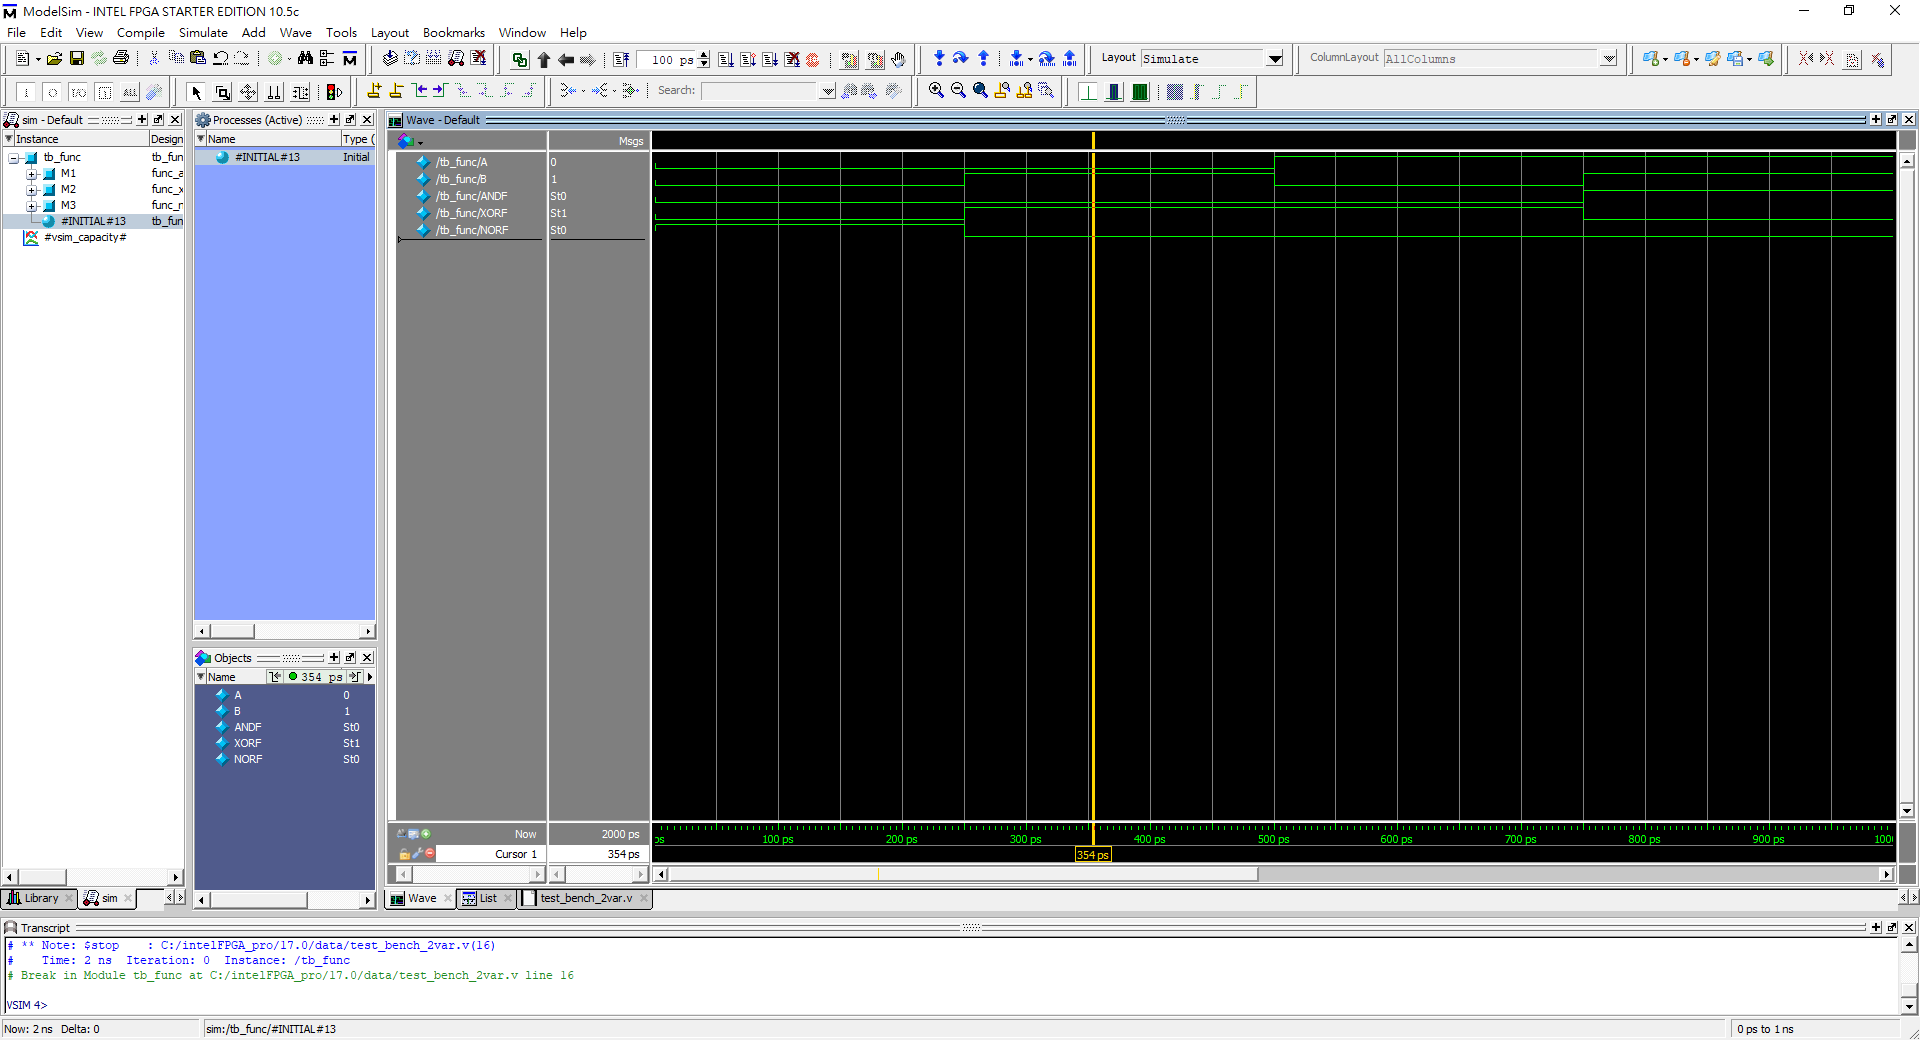
\includegraphics[width=\textwidth, trim=385 175 20 820, clip]{pic/result.png}
    \captionof{figure}{Simulation waveform (cursor at 354 ps: $A=0$, $B=1$, ANDF $=0$, XORF $=1$, NORF $=0$)}
    \label{fig:wave}
\end{figure}

The simulated outputs of all three gates match their truth tables for every input combination.

\section*{6. Problems and Discussion}
% TODO: 補上自己實際遇到的問題與心得（以下是依截圖與講義可以確認的內容）

\begin{itemize}[leftmargin=*]
    \item \textbf{Comparison with the truth tables.} The waveforms of \texttt{ANDF}, \texttt{XORF} and \texttt{NORF} agree with the truth tables for all four input combinations (Tables~\ref{tab:and}--\ref{tab:wave}). Unlike the previous hardware labs, the simulator only shows ideal logic levels (\texttt{St0} / \texttt{St1}, i.e.\ strong 0 / strong 1), so there is no measured voltage to compare.
    \item \textbf{One test bench for several modules.} Instead of writing a separate test bench for each gate, the three modules were included with \texttt{`include} and instantiated in the same \texttt{tb\_func}. They share the same input stimulus, so all outputs can be compared on a single waveform.
    \item \textbf{Initial input combination.} The registers are initialized with \texttt{reg A = 1'b0; reg B = 1'b0;}, so the combination $AB=00$ is applied from 0 to 250 ps without an extra statement in the \texttt{initial} block. The last combination $AB=11$ is held from 750 ps until the simulation stops at 2000 ps.
    \item \textbf{File location.} The \texttt{`include} statements use absolute paths under \texttt{C:/intelFPGA\_pro/17.0/data/}, so the source files must be saved in that directory as the handout requires; otherwise the test bench fails to compile.
\end{itemize}

\section*{Student Feedback (Lab-04)}

This lab was our first time working with Verilog and the simulation software. At first, we spent a lot of time just figuring out how to navigate the tool, and we ran into a few hiccups along the way. For example, we kept getting error messages when compiling. After the TA walked us through it, we realized it was actually a file path issue—definitely a good lesson to pay attention to where we save our files when using this software.

On top of that, we learned how to write a testbench to verify the logic gates and compare the simulated waveforms against the truth table, which really helped us wrap our heads around digital logic design. Once we finished the basic requirements, we wanted to try combining the three separate simulation files into a single test script. That way, it’s much easier to check all three gate outputs at once and see if they’re working properly side by side. After looking up some resources online, we put together two similar versions of the test as our first shot at exploring Verilog on our own.

Overall, this lab gave us a solid starting point with Verilog and the simulation tool, and the TA’s hands-on guidance made the whole process super clear and easy to follow.

\end{document}
